\documentclass[12pt, letterpaper]{report}
\usepackage[margin=1in]{geometry}
\usepackage[utf8]{inputenc}
\usepackage{graphicx}
\usepackage{amsmath}
\usepackage{mathtools}
\usepackage{float}
\usepackage{subfig}
\graphicspath{ {./img/} }
\setlength\parindent{0pt}
\renewcommand{\thesection}{\Roman{section}.}
\renewcommand{\thesubsection}{\alph{subsection}.}


\title{CS1675 - Assignment 8}
\author{Zachary M. Mattis}


\begin{document}

\maketitle

\section{Problem 1 - Bayesian Belief Networks}

\begin{figure}[H]
	\centering
	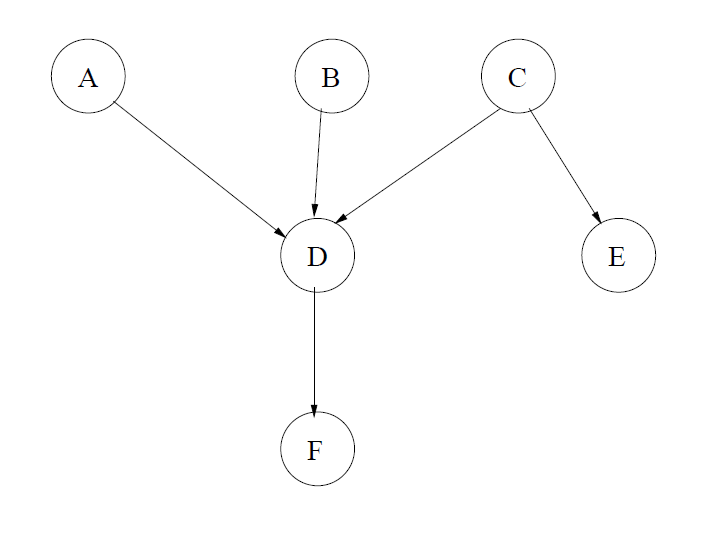
\includegraphics[width=0.4\columnwidth]{bbn.png}
	\caption{BBN}
\end{figure}

% A
\subsection{Blind Solution}

(1) \qquad P(B=T, E=T)


\begin{equation*}
\begin{split}
P(B=T, E=T) &= \sum_{a\in T,F}\sum_{c\in T,F}\sum_{d\in T,F,X}\sum_{f\in T,F} P(A=a,B=T,C=c,D=d,E=T,F=f)\\
&= \sum_{a\in T,F}\sum_{c\in T,F}\sum_{d\in T,F,X}\sum_{f\in T,F}P(F=f|D=d)P(D=d|A=a,B=T,C=c) * \\&\qquad\qquad\qquad\qquad P(E=T|C=c)P(A=a)P(B=T)P(C=c)
\end{split}
\end{equation*}

Computational Cost:

\begin{table}[H]
	\begin{tabular}{ |l|l|r| }
		\hline
		\textbf{Num. Additions} & $(3)(2^3)-1$ & 23 \\
		\hline
		\textbf{Num. Products} & $ [(3)(2^3)][(6-1)]$ & 120 \\
		\hline
	\end{tabular}
	%\caption{Blind Computation Cost}
\end{table}

(2) \qquad Full Joint Distribution


\begin{equation*}
\begin{split}
P &= \sum_{a\in T,F}\sum_{b\in T,F}\sum_{c\in T,F}\sum_{d\in T,F,X}\sum_{e\in T,F}\sum_{f\in T,F} P(A=a,B=b,C=c,D=d,E=e,F=f)\\
&= \sum_{a\in T,F}\sum_{b\in T,F}\sum_{c\in T,F}\sum_{d\in T,F,X}\sum_{e\in T,F}\sum_{f\in T,F} P(F=f|D=d)P(D=d|A=a,B=b,C=c) * \\&\qquad\qquad\qquad\qquad P(E=e|C=c)P(A=a)P(B=b)P(C=c)
\end{split}
\end{equation*}

Computational Cost:

\begin{table}[H]
	\begin{tabular}{ |l|l|r| }
		\hline
		\textbf{Num. Additions} & $(3)(2^5)-1$ & 95 \\
		\hline
		\textbf{Num. Products} & $ [(3)(2^5)][(6-1)]$ & 480 \\
		\hline
	\end{tabular}
	%\caption{Full Joint Computation Cost}
\end{table}


% B
\subsection{Efficient Solution}

(1) \qquad P(B=T, E=T)

\begin{equation*}
\begin{multlined}
P(B=T,E=T) = P(B=T)\sum_{a\in T,F}P(A=a)\sum_{c\in T,F}P(E=T|C=c)P(C=c)* \\
\sum_{d\in T,F,X}P(D=d|A=a,B=T,C=c)\sum_{f\in T,F}P(F=f|D=d)
\end{multlined}
\end{equation*}

Computational Cost:

\begin{table}[H]
	\begin{tabular}{ |l|r| }
		\hline
		\textbf{Num. Additions} & 9\\
		\hline
		\textbf{Num. Products} & 16	\\
		\hline
	\end{tabular}
	%\caption{Full Joint Computation Cost}
\end{table}

Given the reduction in computation complexity and cost for the efficient solution, this approach is much more desirable than the blind solution.


\section{Problem 2 - Pneumonia Diagnosis}

% A
\subsection{ML Estimation}

\begin{table}[H]
	\centering
	\begin{tabular}{ |r|r|r| }
		\hline
		& \textbf{T} & \textbf{F} \\
		\hline
		\textbf{Fever} & 0.9 & 0.1 \\
		\hline
		\textbf{Paleness} & 0.7 & 0.3 \\
		\hline
		\textbf{Cough} & 0.9 & 0.1 \\
		\hline
		\textbf{HighWBCcount} & 0.8 & 0.2 \\
		\hline
	\end{tabular}
	\caption{$P(Parameters \mid Pneumonia = T)$}
\end{table}


\begin{table}[H]
	\centering
	\begin{tabular}{ |r|r|r| }
		\hline
		& \textbf{T} & \textbf{F} \\
		\hline
		\textbf{Fever} & 0.6 & 0.4 \\
		\hline
		\textbf{Paleness} & 0.5 & 0.5 \\
		\hline
		\textbf{Cough} & 0.1 & 0.9 \\
		\hline
		\textbf{HighWBCcount} & 0.5 & 0.5 \\
		\hline
	\end{tabular}
	\caption{$P(Parameters \mid Pneumonia = F)$}
\end{table}


% B
\subsection{Fever, !Paleness, Cough, !HighWBCcount}

$P(Pneumonia = T | Fever = T,Paleness = F,Cough = T,HighWBCcount = F) = 0.2351$

% C
\subsection{Fever, ?Paleness, Cough, ?HighWBCcount}

$P(Pneumonia = T | Fever = T,Cough = T) = 0.0539$

% D
\subsection{Current Symptoms}

\begin{verbatim}
main7_2inference.m
\end{verbatim}

\end{document}